\documentclass[xetex]{beamer}

\mode<presentation> {
  \usetheme{Frankfurt}
  \setbeamercovered{transparent}
}

\usepackage{xunicode}
\usepackage{xltxtra}
\usepackage[czech]{babel}
\usepackage{palatino}
\usepackage{graphicx}
\usepackage{textpos}

%\usepackage{listings}
%\lstset{language=bash,
%        numbers=left,
%       numberstyle=\tiny,
%        showstringspaces=false,
%        aboveskip=-40pt,
%        frame=leftline
%        }

\title{Otevřená bezpečnost}

\author{Ondřej Profant}
\institute[Piráti]{Česká pirátská strana\\Cybesecurity 2014}

\date{Verze: \today}

\begin{document}

%\begin{frame}
%  \begin{textblock*}{0cm}(-1.2cm,-4.2cm)
%  
\includegraphics[scale=1.2]{images/intro.jpg}
%  \end{textblock*}
%\end{frame}

\begin{frame}
  \titlepage
\end{frame}

\section{Témata}

\begin{frame}
	\frametitle{Témata}
	\begin{itemize}
		\item Paradigmata
		\item Lidské zdroje
		\item Předsudky
	\end{itemize}
\end{frame}	

\section{Bezpečnost}

\begin{frame}
	\frametitle{Bezpečnost je kritická}
	Bezpečnost je zcela kritická, zároveň však překvapivě opomíjená.

	\medskip

	Ve skutečnosti je totiž opomíjená ve většině procesu realizace projektu:

	\begin{itemize}
		\item návrh, 
		\item implementace, 
		\item testování.
	\end{itemize}

	\medskip

\end{frame}

\begin{frame}

\bigskip

I ty největší projekty mají chyby (v kódu). Např. LinkedIn, Github, Seznam.

\bigskip

Mnohdy znamé. Ať už teoreticky, či prakticky.

\bigskip

(Oprávněná) obhajoba: nedostatek expertů, času, zdrojů
\end{frame}

\begin{frame}
	\frametitle{Bezpečnost}

	Oblíbený úskok:

	\bigskip

	\begin{block}{Security through obscurity}
	Bezpečné je to, co je bezpečné (dokázané, testované, odladěné).

	\medskip

	Nikoliv to, co je skryté.
	\end{block}
\end{frame}

\section{Otevřenost}

\begin{frame}
	\frametitle{Otevřenost}
	OSS projekty tu jsou a jsou minimálně stejně bezpečné jak jejich proprietární protějšky.

	\bigskip

	V čem otevřenost pomůže:
	\begin{itemize}
		\item Tlak na preciznost.
		\item Širší diskuse.
		\item Lepší integrace dalších otevřených řešení.
	\end{itemize}

	\bigskip

	V čem neuškodí:
	\begin{itemize}
		\item Bezpečnost – pokud chyba existuje, tak si jí útočník najde (pokud chce opravdu útočit).
	\end{itemize}
\end{frame}

\begin{frame}
	\frametitle{Otevřenost}
	Přínos pro všechny.

	\bigskip

	Pokud i ostatním „pomůžete“ s bezpečností, bude celé prostředí stabilnější. 
	Příkladem jsou DDOS.

	\medskip

	Ad absurdum: přece byste nechtěli obchodovat v anarchii.
\end{frame}

\section{Příklad}
% https://plus.google.com/113127038390856514619/posts/D3YWhgjw8KX
\begin{frame}
	\frametitle{Příklad}

	Seznam.cz a zasílaní hesel v nešifrované podobě.

	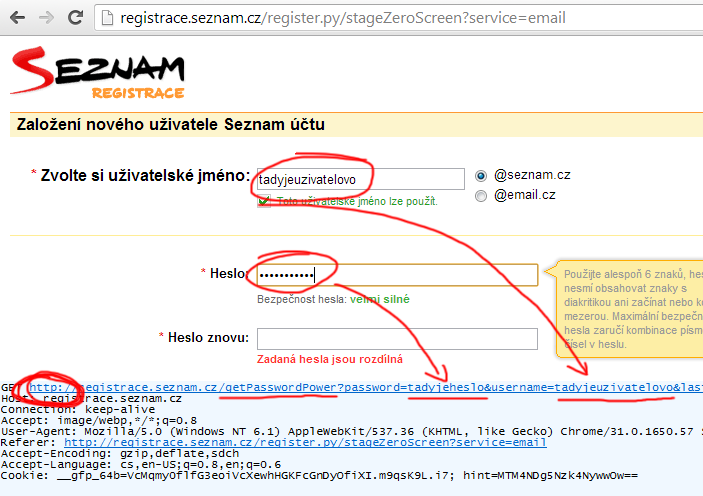
\includegraphics[scale=0.3]{pic/seznam.png}
\end{frame}

\begin{frame}
	Ilustruje většinu zmíněných problémů:
	\begin{itemize}
		\item Kód převážně pro UI
		\item Kód doplněn později
		\item Odeslání formuláře se již provedlo bezpečně
		\item Nestandardní řešení (běžné je ověřit přímo v JS, nikoliv na serveru)
	\end{itemize}
\end{frame}

\section{Modely}

\begin{frame}
	\frametitle{Bug bounty program}
	Odměna za nalezení chyby.

	\medskip

	Využívá například:
	\begin{itemize}
		\item Adobe
		\item Apple
		\item Avast
		\item Github
		\item Google
	\end{itemize}
\end{frame}

\begin{frame}
	\frametitle{Další modely}
	
	Do budoucna je třeba motivovat chytré a schopné lidi,
	aby raději spolupracovali, než „bojovali“.

	\bigskip

	Dobré příklady existují, 
	avšak občas jsou ubíjeny starými paradigmaty.
\end{frame}

\section{Závěr}

\begin{frame}
	Děkuji za pozornost.

	\bigskip
	
	Doplňující otázky?

	\bigskip

	\bigskip

	\scriptsize
	Copyleft Ondřej Profant, 2014. 
	Všechna práva vyhlazena. Sdílejte, upravujte a~nechte sdílet za stejných podmínek. 

	\bigskip

	Prezentace v~úplné formě\footnote{i se zdrojovými kódy} na:\\ 
	\url{https://www.github.com/kedrigern/prezentace-cs}.

	\bigskip

	Mail: ondrej.profant -at- pirati.cz 
\end{frame}

\end{document}
